\section{Внутренние форматы хранения данных}
\setcounter{figure}{0}

% The 3-Clause BSD License

В данной работе используется комбинация из различных структур данных, 
объединённых в единую систему.
Полная схема структур и их связей представленна на рис. \ref{overall_data_structure}

\begin{figure}[hpt!]
    \centering
    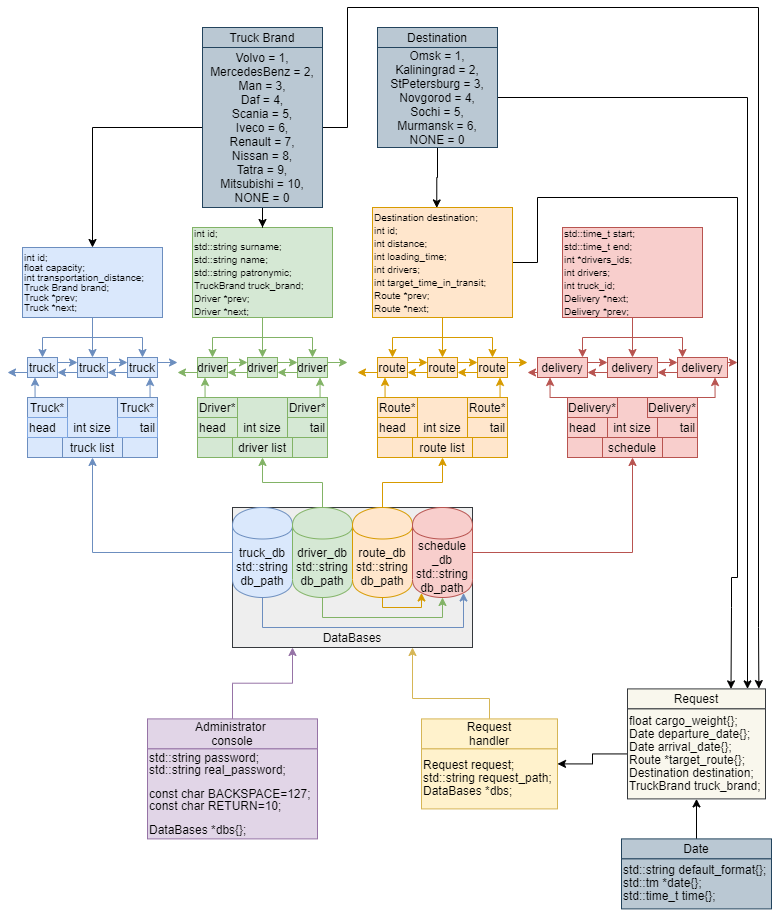
\includegraphics[width=1\linewidth]{photo/overall_data_structure}
    \caption{Обзорная диаграмма структур данных программы}
    \label{overall_data_structure}
\end{figure}

\newpage

\subsection{Структура данных двусвязный список}

В работе предпологается использование структуры данных "список".
Список --- структура данных, состоящая из элементов, 
содержащих помимо собственных данных ссылки на 
следующий и/или предыдущий элемент списка \cite{list_defenition}.

Для работы был вабран вариант с двунаправленым списком, 
где каждый узел имеет указатель на следующий и на предыдущий элементы.
Схема двунаправленного списка показана на рис. \ref{list_schema}.

\begin{figure}[hpt!]
    \centering
    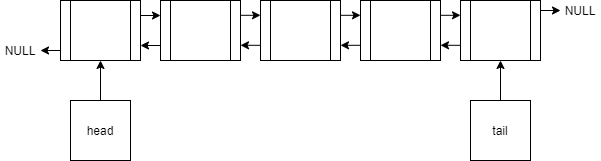
\includegraphics[width=1\linewidth]{photo/list_schema}
    \caption{Схема структуры данных двусвязный список}
    \label{list_schema}
\end{figure}

\subsection{TruckBrand}

Структурой данных \textbf{перечисление} представленны марки грузовиков.
Здесь содержаться все возможные значения марок грузовиков транспортной компании. 

Схема представлена на рис. \ref{truck_brand}

% рисунок

\subsection{Destination}


Возможные маршруты поставки содержаться в структуре данных  \textbf{перечисление}.
Здесь содержаться все возможные значения маршрутов транспортной компании. 

Схема представлена на рис. \ref{destination}

% рисунок

\subsection{Truck}

Представление грузовика в памяти программы выполнено в виде структуры Truck со следующими полями:

\begin{itemize}
    \item 1
\end{itemize}

Схема на рис. \ref{truck}.

% рисунок

\subsection{TruckList}

Для управления списком грузовиков используется структура TruckList со следующими полями:

\begin{itemize}
    \item 1
\end{itemize}

Структура так же содержит методы для управления списком.

Схема на рис. \ref{truck_list}.

% рисунок

\subsection{TruckDataBase}

Для управления базой данных грузовиков, 
её загрузки и обновления, 
используется структура TruckDataBase со следующими полями: 

\begin{itemize}
    \item 1
\end{itemize}

Структура так же содержит методы для управления базой данных.

Схема на рис. \ref{truck_db}.

% рисунок

\subsection{Route}

Представление маршрута в памяти программы выполнено в виде структуры Route со следующими полями:

\begin{itemize}
    \item 1
\end{itemize}

Схема на рис. \ref{route}.

% рисунок

\subsection{RouteList}

Для управления списком маршрутов используется структура RouteList со следующими полями:

\begin{itemize}
    \item 1
\end{itemize}

Структура так же содержит методы для управления списком.

Схема на рис. \ref{route_list}.

% рисунок

\subsection{RouteDataBase}

Для управления базой данных маршрутов, 
её загрузки и обновления, 
используется структура RouteDataBase со следующими полями: 

\begin{itemize}
    \item 1
\end{itemize}

Структура так же содержит методы для управления базой данных.

Схема на рис. \ref{route_db}.

% рисунок

\subsection{Driver}

Представление водителя в памяти программы выполнено в виде структуры Driver со следующими полями:

\begin{itemize}
    \item 1
\end{itemize}

Схема на рис. \ref{driver}.

% рисунок

\subsection{DriverList}

Для управления списком водителей используется структура DriverList со следующими полями:

\begin{itemize}
    \item 1
\end{itemize}

Структура так же содержит методы для управления списком.

Схема на рис. \ref{driver_list}.

% рисунок

\subsection{DriverDataBase}

Для управления базой данных водителей, 
её загрузки и обновления, 
используется структура DriverDataBase со следующими полями: 

\begin{itemize}
    \item 1
\end{itemize}

Структура так же содержит методы для управления базой данных.

Схема на рис. \ref{driver_db}.

% рисунок

\subsection{Delivery}

Представление поставки в памяти программы выполнено в виде структуры Delivery со следующими полями:

\begin{itemize}
    \item 1
\end{itemize}

Схема на рис. \ref{delivery}.

% рисунок

\subsection{Schedule}

Для управления списком поставок используется структура Schedule со следующими полями:

\begin{itemize}
    \item 1
\end{itemize}

Структура так же содержит методы для управления списком.

Схема на рис. \ref{schedule}.

% рисунок

\subsection{ScheduleDataBase}

Для управления базой данных поставок, 
её загрузки и обновления, 
используется структура DriverDataBase со следующими полями: 

\begin{itemize}
    \item 1
\end{itemize}

Структура так же содержит методы для управления базой данных.

Схема на рис. \ref{schedule_db}.

% рисунок

\subsection{DataBases}
\subsection{AdministratorConsole}
\subsection{Date}
\subsection{Request}
\subsection{RequestHandler}
